% !TeX encoding = utf8
% !TeX root = Rename
%
%%%%%%

\Mysection{Introduction}

\STANDARD{Introduction I}
{
	\begin{itemize}
		\item The project focuses on designing an automatic car license plate detection system using the Nvidia Jetson Nano.
		\item  License plates are detected using ML models (CNN) deployed on embedded devices. \cite{Tan+22} \cite{jocher2023ultralytics,Cor21}.		
		\item Application: Places with high vehicle throughput such as airport departures, where manual verification is inefficient and error-prone. 
		 
	\end{itemize}
	
}

\Mysection{Description of Application}
	
\STANDARD{Description of Application I}
{
	\begin{itemize}
		\item \textbf{Target deployments:} Airport curbside (drop-off time control) and parking facilities (paid stay management).
		\item \textbf{Core idea:} detect the license plate at \textbf{entry} and \textbf{exit} using a camera + Jetson Nano, and use timestamps to compute dwell time.
		\item \textbf{Edge-first operation:} Recognition and decision making run locally enabling low latency. Reduced dependence on centralized servers.
		\item \textbf{Operator-specific configuration (before delivery):} the airport/parking authority provides billing requirements (tariff, grace period, rounding rules); we configure the system accordingly and deploy it.
		\item \textbf{System output:} validated plate ID, entry/exit events, and a fee/permission decision shown on a display.
	\end{itemize}
}

\STANDARD{Description of Application II}
{
	\begin{itemize}
		\item \textbf{Entry flow:} camera captures vehicle $\rightarrow$ YOLO detects license plate $\rightarrow$ OCR reads text $\rightarrow$ store \texttt{(plate\_id, entry\_timestamp)} in database.
		\item \textbf{Exit flow:} detect plate again $\rightarrow$ retrieve \texttt{entry\_timestamp} $\rightarrow$ compute dwell time \texttt{(exit - entry)}.
		\item \textbf{Billing logic (configured per operator):} apply provided parameters (grace minutes, \euro{}/hour tariff, rounding) $\rightarrow$ compute amount due.
		\item \textbf{Decision \& display:} show “free exit” or “payment required” with the calculated amount due.
		\item \textbf{Logging:} write \texttt{exit\_timestamp} and fee outcome for auditing and analytics.
	\end{itemize}
}

\STANDARD{Description of Application III}
{
	\begin{figure}
		\centering
		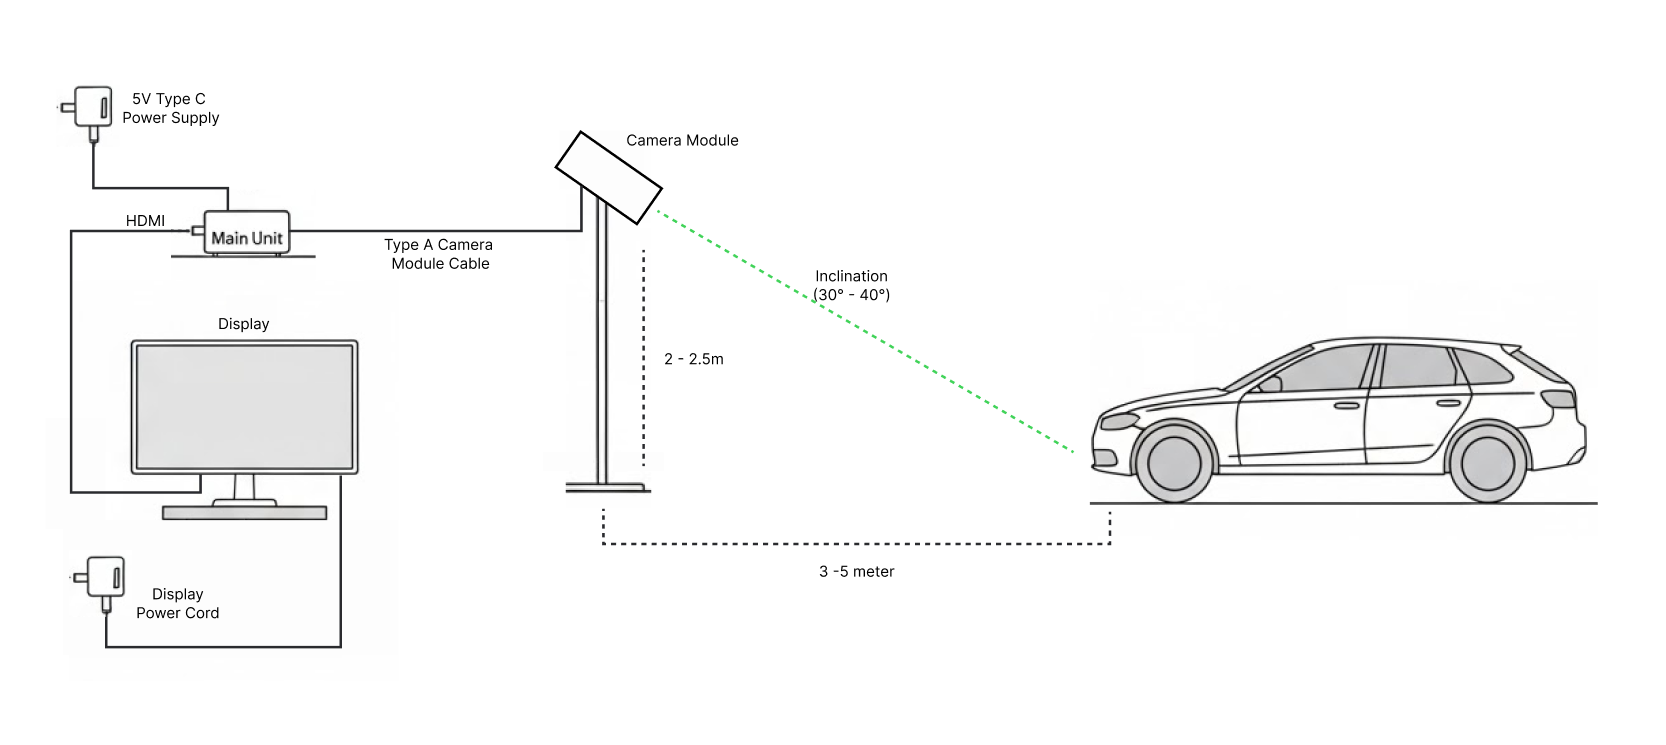
\includegraphics[width=1.0\textwidth]{img/lp_setup.png}
		\caption{ License Plate Detection System.}
	\end{figure}
}

\Mysection{Challenges and Solutions}

% ==============================================================================
% SLIDE 1: MEMORY CHALLENGE
% ==============================================================================
\STANDARD{Challenge 1: System Memory Exhaustion}
{
	\renewcommand{\arraystretch}{1.5} 
	\small 
	
	\noindent
	\begin{tabular}{|p{0.48\linewidth}|p{0.48\linewidth}|}
		\hline
		\cellcolor{red!40!black}\textbf{\color{white} The Problem} & 
		\cellcolor{blue!40!black}\textbf{\color{white} The Engineered Solution} \\ 
		\hline
		\cellcolor{gray!10}
		\textbf{Conflict: Unified Memory Bottleneck} \newline
		The Jetson Nano shares a single 4GB RAM pool between the CPU and GPU.
		\newline \newline
		$\bullet$ \textbf{OS Overhead:} Ubuntu 18.04 consumes $\approx$ 1.2 GB. \newline
		$\bullet$ \textbf{AI Load:} YOLOv5 + EasyOCR required $\approx$ 3.3 GB during initialization.
		\newline \newline
		\textit{Impact:} Demand (4.5 GB) exceeded physical limits. The Linux kernel invoked the OOM Killer and terminated the process instantly.
		& 
		\cellcolor{gray!10}
		\textbf{Solution: Hybrid Memory Architecture}:
		\newline \newline
		$\bullet$ \textbf{Virtual Expansion:} Configured a \textbf{6GB Swap Partition} on an external SSD to offload inactive OS pages, keeping physical RAM free for inference. \newline
		\newline			
		$\bullet$ \textbf{Compute Isolation:} Forced OCR to run on the \textbf{CPU} (\texttt{gpu=False}). This reserves the limited GPU VRAM entirely for YOLO detection. \\
		\hline
	\end{tabular}
}

% ==============================================================================
% SLIDE 2: SOFTWARE CHALLENGE
% ==============================================================================
\STANDARD{Challenge 2: Legacy Software Ecosystem}
{
	\renewcommand{\arraystretch}{1.5}
	\small
	
	\noindent
	\begin{tabular}{|p{0.48\linewidth}|p{0.48\linewidth}|}
		\hline
		\cellcolor{red!40!black}\textbf{\color{white} The Problem} & 
		\cellcolor{blue!40!black}\textbf{\color{white} The Engineered Solution} \\ 
		\hline
		\cellcolor{gray!10}
		\textbf{Conflict: Dependency Conflicts} \newline
		The Jetson Nano relies on JetPack 4.6 (Ubuntu 18.04), which locks the environment to \textbf{Python 3.6}.
		\newline \newline
		$\bullet$ \textbf{Incompatibility:} State-of-the-art libraries (Ultralytics YOLOv8, Pandas 2.0) require Python 3.8+ and modern C++ compilers, causing installation failures. \newline
		$\bullet$ \textbf{Deprecated APIs:} The \texttt{Pillow} image library recently removed attributes (like \texttt{ANTIALIAS}) used by older Jetson inference tools, causing runtime crashes.
		& 
		\cellcolor{gray!10}
		\textbf{Solution: Cross-Compilation Workflow} \newline
		We bypassed the OS limitations using an external pipeline:
		\newline \newline
		$\bullet$ \textbf{TensorRT Export:} Instead of running PyTorch natively, we trained the model on a PC, exported it to \textbf{ONNX}, and cross-compiled it into a \textbf{.engine} binary specifically optimized for the Nano's Maxwell GPU. \newline
		$\bullet$ \textbf{Monkey Patching:} We developed a custom initialization script that injects code at runtime to manually map old API calls to their new locations, preventing crashes in legacy libraries. \\
		\hline
	\end{tabular}
}

% ==============================================================================
% SLIDE 3: REMOTE DEV CHALLENGE
% ==============================================================================
\STANDARD{Challenge 3: Remote Development Breakdown}
{
	\renewcommand{\arraystretch}{1.5}
	\small
	
	\noindent
	\begin{tabular}{|p{0.48\linewidth}|p{0.48\linewidth}|}
		\hline
		\cellcolor{red!40!black}\textbf{\color{white} The Problem} & 
		\cellcolor{blue!40!black}\textbf{\color{white} The Engineered Solution} \\ 
		\hline
		\cellcolor{gray!10}
		\textbf{Conflict: glibc Version Lock} \newline
		In 2024, Microsoft updated the VS Code Remote Server to require \textbf{glibc 2.28} or higher.
		\newline \newline
		$\bullet$ \textbf{The Lockout:} The Jetson Nano's OS is pinned to \textbf{glibc 2.27}. \newline
		$\bullet$ \textbf{Impact:} Standard SSH connections failed with "OS Not Supported" errors, blocking all direct code editing and file transfer capabilities on the device.
		& 
		\cellcolor{gray!10}
		\textbf{Solution: SSH-FS Protocol Switch} \newline
		We architected a workaround that avoids running binary agents on the Jetson:
		\newline \newline
		$\bullet$ \textbf{SFTP Mounting:} We switched to the \textbf{SSH FS} extension, which mounts the Jetson's external SSD (/media/myssd) as a local network drive on the development laptop. \newline
		$\bullet$ \textbf{Benefit:} This protocol relies purely on standard SFTP, which does not check the glibc version, allowing full real-time coding access despite the OS obsolescence. \\
		\hline
	\end{tabular}
}

% ==============================================================================
% SLIDE 4: LOGIC CHALLENGE
% ==============================================================================
\STANDARD{Challenge 4: Latency \& Logic}
{
	\renewcommand{\arraystretch}{1.5}
	\small
	
	\noindent
	\begin{tabular}{|p{0.48\linewidth}|p{0.48\linewidth}|}
		\hline
		\cellcolor{red!40!black}\textbf{\color{white} The Problem} & 
		\cellcolor{blue!40!black}\textbf{\color{white} The Engineered Solution} \\ 
		\hline
		\cellcolor{gray!10}
		\textbf{Conflict: Hardware Constraints} \newline
		$\bullet$ \textbf{Latency:} Running the heavy Optical Character Recognition (OCR) model on every video frame dropped performance to an unusable \textbf{1 FPS} due to CPU bottlenecks. \newline
		$\bullet$ \textbf{Single-Camera Limit:} A standard parking system uses two cameras (Entry/Exit). With only one camera, the system lacks a physical sensor trigger to determine when a car has left the frame.
		& 
		\cellcolor{gray!10}
		\textbf{Solution: State Machine Heuristics} \newline
		We developed a specialized algorithm to compensate:
		\newline \newline
		$\bullet$ \textbf{Cooldown Timer:} We implemented a logic gate that pauses the OCR engine for \textbf{3 seconds} after a successful read. This keeps the video smooth by running only the lightweight Detector during the cooldown. \newline
		$\bullet$ \textbf{Last-Seen Algorithm:} The system updates a timestamp for every frame the car is visible. The billing logic defines Exit Time as the exact moment the timestamp ceases to update. \\
		\hline
	\end{tabular}
}

\Mysection{Results}		

\STANDARD{System Demonstration Video}
{

	
	\vspace{0.2cm}
	\textit{Embedded video demonstrating real-time license plate detection and decision logic.}
}